\chapter[Gamma-Konvergenz: Eine Einführung]{\(\Gamma\)-Konvergenz: Eine Einführung}{\label{ch:gamma}}
\pgfsetfillopacity{0.1}\colorbox{generalYellow}{\begin{minipage}{16cm}{\textcolor{black}{\pgfsetfillopacity{1}}{\label{not3}}}
\textbf{Notation:} Im Folgenden sei stets:
\begin{itemize}
    \item \(\mathcal{N}(x)\) der Umgebungsfilter eines Punktes x in einem topologischen Raum \((X,\mathcal{T})\); im Folgenden betrachten wir dann jeweils einen Repräsentanten einer inkludierten offenen Umgebung von x.
\end{itemize}
\end{minipage}}\\

Wir haben in \ref{sec:calcvar} kennengelernt, wie man Minimierer/Maximierer von Funktionalen findet. Doch was passiert, wenn man Modelle betrachtet, die von einem Parameter abhängen? Wir sind an dem asymptotischen Verhalten interessiert, welches beantwortet, was geschieht, wenn wir den Parameter in der Minimierungsfolge des parametrisierten Funktionals gegen 0 streben lassen.\\
Dieser Fall ist nicht gerade selten und der Einfluss, den dieser auf Probleme nimmt, ist im Allgemeinen nicht zu unterschätzen. Es hat sich deshalb hierfür eine eigene analytische Theorie entwickelt. Die Rede ist von der \(\Gamma\)-Konvergenz, die wir im Folgenden nun einführen wollen, da wir bei der Modellierung von Phasenübergängen mit dem wie eben beschriebenen parametrisierten Fall arbeiten werden.\\
Eine weitere Frage, der wir uns kurz am Ende des Kapitels widmen werden, ist, wie man variationelle Probleme lösen kann, deren Funktional(e) nicht unterhalbstetig ist/sind.\\

\section[Analysis parametrisiert variationeller Probleme: Gamma-Konvergenz]{Analysis parametrisiert variationeller Probleme: \(\Gamma\)-Konvergenz}{\label{sec:anagamma}}
Für die Untersuchung derartiger mathematischer Probleme behelfen wir uns der von Ennio De Giorgi eingeführten Theorie der \(\Gamma\)-Konvergenz. Als einer der größten\\ Mathematiker aller Zeiten für die Forschung im Bereich partielle Differential-\\gleichungen, führte er in den Jahren 1975-1983 zunächst den Begriff der "G-Konvergenz" ein, da die Theorie für die Greensche Funktion entwickelt wurde \cite{BioDeGiorgi}. Nach Verallgemeinerung etablierte sich jedoch \(\Gamma\)-Konvergenz als Bezeichnung:\\[0.5cm]
\pgfsetfillopacity{0.1}\colorbox{generalYellow}{\begin{minipage}{16cm}{\textcolor{black}{\pgfsetfillopacity{1}}{\label{def3.1}}}
\textbf{Definition 3.1 (\(\Gamma\)-Konvergenz, Notation aus \cite{MasoGamma}[Definition 4.1]):} Sei \((X,\mathcal{T})\) ein topologischer Raum. Betrachte für \(h \in \mathbb{N}\) die Funktionale \(\mathcal{F},\mathcal{F}_h: X \to \overline{\mathbb{R}}\). Dann ist \(\mathcal{F}_h\) \(\Gamma\)-konvergent gegen \(\mathcal{F}\) \(:\Leftrightarrow\)
\begin{equation}
    \sup_{U \in \mathcal{N}(x)} \limsup_{h \to \infty} \inf_{y \in U} \mathcal{F}_h(y) \leq \Gamma-\lim_{h \to \infty} \mathcal{F}_h = \mathcal{F} \leq \sup_{U \in \mathcal{N}(x)} \liminf_{h \to \infty} \inf_{y \in U} \mathcal{F}_h(y)\,\, \forall x \in X,
\end{equation}
bzw. kurz:
\begin{equation}
    \Gamma-\limsup_{h \to \infty} \mathcal{F}_h \leq \mathcal{F} \leq \Gamma-\liminf_{h \to \infty} \mathcal{F}_h.
\end{equation}
Ist \(X\) ein erstabzählbarer (T2)-Raum (die Forderung nach dem 1.AA kann man für \(\Gamma\)-Konvergenz etwas abschwächen, siehe \ref{sec:gammatopo}), so ist \(\Gamma\)-Konvergenz äquivalent definiert als:
\begin{equation}
    \forall x_h \stackrel{h \to \infty}{\to} x \in X: \, \limsup_{h \to \infty} \mathcal{F}_h (x_h) \leq \mathcal{F}(x) \leq \liminf_{h \to \infty} \mathcal{F}_h (x_h).
\end{equation}
\end{minipage}}\\

\textbf{Bemerkung:} Es ist nicht einschränkend, die Definition "nur" für einen diskreten Fall zu verfassen, denn der kontinuierliche Fall (für den wir uns, wie eingangs schon motiviert, interessieren) übersetzt sich direkt wie folgt: Für \(h \to \infty\) fordert man, dass \(\mathbb{R}^+ \supset \{\epsilon_h\} \to 0^+\) und betrachtet dann \(\mathcal{F}_{{\epsilon}_h}\).\\

Wir werden im Folgenden den Begriff der gleichgradigen Koerzivität benötigen:\\
\(\mathcal{F}_h\) ist gleichgradig-koerziv auf \(X \, :\Leftrightarrow\)
\begin{equation}
    \forall t \in \mathbb{R} \, \exists K_t \subset X \text{ abgeschlossen, abzählbar kompakt} \, \forall h \in \mathbb{N} \, : \, \{\mathcal{F}_h \leq t\} \subseteq K_t.
\end{equation}
Vergleicht man diese Definition mit der direkten Methode [\ref{theo2.8}, Satz 2.8], so ist intuitiv klar, warum wir diese Eigenschaften benötigen werden und tatsächlich kann man auch zeigen:\\[0.5cm]
\pgfsetfillopacity{0.1}\colorbox{generalYellow}{\begin{minipage}{16cm}{\textcolor{black}{\pgfsetfillopacity{1}}{\label{prop3.2}}}
\textbf{Proposition 3.2 (\cite{MasoGamma}[Proposition 7.7]):} \(\mathcal{F}_h\) ist gleichgradig-koerziv auf \(X\) \(\Leftrightarrow\)
\begin{equation}
    \exists \psi : X \to \overline{\mathbb{R}} \text{ unterhalbstetig, koerziv} \, \forall h \in \mathbb{N} \, : \, \mathcal{F}_h \geq \psi \text{ in }X.
\end{equation}
\end{minipage}}\\

\textsc{Beweis:} Betrachte
\begin{equation}
    \psi(x) := \inf \{s \in \mathbb{R} \, | \, x \in K_t \forall t > s\},
\end{equation}
wobei \(\inf \emptyset := \infty\) und wende Beweismethoden sehr ähnlich wie der für den Beweis der direkten Methode [\ref{theo2.8}, Satz 2.8] an. \QEDB

Es stellt sich nun natürlich die Frage, warum wir an genau dieser Konvergenzart interessiert sind, wenn wir die eingängliche Frage dieses Kapitels beantworten wollen. Die wesentlichen zwei Hauptargumente liefert die folgende Proposition:\\[0.5cm]
\pgfsetfillopacity{0.1}\colorbox{generalYellow}{\begin{minipage}{16cm}{\textcolor{black}{\pgfsetfillopacity{1}}{\label{prop3.3}}}
\textbf{Proposition 3.3 (\cite{MasoGamma}[Proposition 6.8, Theorem 7.8]):} Sei \((X,\mathcal{T})\) ein topologischer Raum. Dann gilt:
\begin{enumerate}
    \item \(\Gamma-\liminf_{h \to \infty} \mathcal{F}_h\) und \(\Gamma-\limsup_{h \to \infty} \mathcal{F}_h\) sind unterhalbstetig auf \(X\),
    \item Ist \(\mathcal{F}_h\) gleichgradig-koerziv auf \(X\), so sind \(\Gamma-\liminf_{h \to \infty} \mathcal{F}_h\) und \(\Gamma-\limsup_{h \to \infty} \mathcal{F}_h\) koerziv und es gilt:
    \begin{equation}{\label{eq3.7}}
        \min_{x \in X} \Gamma-\liminf_{h \to \infty}\mathcal{F}_h(x) = \liminf_{h \to \infty} \inf_{x \in X} \mathcal{F}_h(x).
    \end{equation}
    Falls \(\mathcal{F}_h \stackrel{\Gamma}{\to} \mathcal{F}\) in \(X\), dann ist \(\mathcal{F}\) koerziv und es gilt:
    \begin{equation}{\label{eq3.8}}
        \min_{x \in X} \mathcal{F}(x) = \lim_{h \to \infty} \inf_{x \in X} \mathcal{F}_h(x).
    \end{equation}
\end{enumerate}
\end{minipage}}\\

\textsc{Beweis:}
\begin{enumerate}
    \item Folgt direkt aus der Tatsache, dass:
    \begin{equation}
        \sup_{U \in \mathcal{N}(x)} f(U) \text{ mit }f: \mathcal{T}_{sub} \supset \Omega \to \overline{\mathbb{R}},
    \end{equation}
    unterhalbstetig auf \(X\) ist.
    \item Die Koerzivität des \(\Gamma\)-Liminf/-Limsup folgt direkt aus dessen Definition und [\ref{prop3.2}, Proposition 3.2]. Wir beweisen nun also \eqref{eq3.7}:
    \begin{itemize}
        \item "\(\geq\)": Folgt direkt aus der Definition des \(\Gamma\)-Liminf;
        \item "\(\leq\)": Ist die rechte Seite \(\infty\), so ist nichts zu zeigen. Angenommen also, sie ist \(< \infty\). Dann können wir \(t \in \mathbb{R}\) wählen, sodass für eine Teilfolge \(\mathcal{F}_{h_k}\)
        \begin{equation}
            \lim_{k \to \infty} \inf_{x \in X} \mathcal{F}_{h_k}(x) = \liminf_{h \to \infty} \inf_{x \in X} \mathcal{F}_h(x) < t,
        \end{equation}
        sowie
        \begin{equation}
            \inf_{x \in X} \mathcal{F}_{h_k}(x) < t
        \end{equation}
        gilt für alle \(k \in \mathbb{N}\). Damit sind die Subniveaumengen \(\{\mathcal{F}_{h_k} \leq t\}\) nicht leer und es gilt:
        \begin{equation}
            \inf_{x \in X} \mathcal{F}_{h_k}(x) \stackrel{gl.Koer.}{=} \inf_{x \in K_t} \mathcal{F}_{h_k}(x) \, \forall k \in \mathbb{N}.
        \end{equation}
        Die Behauptung folgt nun aus der Definition des \(\Gamma\)-Liminf.
    \end{itemize}
    \eqref{eq3.8} folgt aus \eqref{eq3.7} und der Definition des \(\Gamma\)-Limsup. \QEDB
\end{enumerate}

Bevor wir uns nun etwas Existenztheorie zuwenden, präsentieren wir hier als erste Warnung ein Beispiel, dass sich \(\Gamma\)-Konvergenz \textbf{nicht} wie punktweise Konvergenz verhält:\\[0.5cm]
\pgfsetfillopacity{0.1}\colorbox{generalYellow}{\begin{minipage}{16cm}{\textcolor{black}{\pgfsetfillopacity{1}}{\label{ex3.4}}}
\textbf{Beispiel 3.4 (\cite{MasoGamma}[Example 6.6]):} Sei \(A\) eine offene Teilmenge des \(\mathbb{R}^n\), \(\{a_h\} \subset L^{\infty}(A)\). Wir betrachten nun das Integralfunktional:
\begin{equation}
    \mathcal{F}_h : L^2(A) \to \mathbb{R}, \, \mathcal{F}_h(u) := \int_A a_h u^2  \, d\lambda^n(x).
\end{equation}
Angenommen, es existieren \(0 < C_1 \leq C_2\), sodass \(C_1 \leq a_h \leq C_2\) \(\lambda^n\)-f.ü. gilt und es existieren \(a,b \in L^{\infty}(A)\) mit
\begin{equation}
    (a_h \to a \, \land \, \frac{1}{a_h} \stackrel{*}{\rightharpoonup} \frac{1}{b}).
\end{equation}
Sind \(\mathcal{F},\mathcal{G} : L^2(A) \to \mathbb{R}\) zwei Funktionale definiert durch:
\begin{equation}
    \mathcal{F}(u) := \int_A a u^2 \, d\lambda^n(x), \, \, \mathcal{G}(u) := \int_A b u^2 \, d\lambda^n(x),
\end{equation}
dann gilt:
\begin{equation}
    \mathcal{F}_h \to \mathcal{F} \text{ in }L^2(A), \text{aber } \GaLim \mathcal{F}_h = \mathcal{F}, \, \GaLimW \mathcal{F}_h = \mathcal{G}. 
\end{equation}
\end{minipage}}\\

\textsc{Beweis:} \begin{itemize}
    \item Der erste Grenzwert folgt direkt aus einer majorisierten Konvergenz.
    \item Der zweite Grenzwert folgt aus der gleichgradigen Beschränktheit von \(\mathcal{F}_h\):
\begin{equation}
    |\mathcal{F}_h(x)| \leq C_2 \int_A u^2 \,d\lambda^n(x) \leq C=C(C_2,A)
\end{equation}
    \item Nun der dritte Grenzwert: 
    \begin{itemize}
        \item \(\Gamma_w\)-Limsup: Sei dazu \(u_h := \frac{bu}{a_h}\). Dann gilt:
\begin{equation}{\label{eq3.18}}
    \mathcal{F}_h (u_h) \stackrel{h \to \infty}{\to} \mathcal{G}(u).
\end{equation}
Wähle nun \(h\) groß genug, dass \(u_h \in U\) für eine Umgebung \(U\) von \(u\) in der schwachen Topologie, sodass folgt:
\begin{equation}
    \limsup_{h \to \infty} \inf_{v \in U} \mathcal{F}_h (v) \leq \lim_{h \to \infty} \mathcal{F}_h (u_h) \stackrel{\eqref{eq3.18}}{=} \mathcal{G}(u).
\end{equation}
\item \(\Gamma_w\)-Liminf: Folgt aus:
\begin{equation}
    a_h v^2 \geq - a_h u_h^2 + 2buv
\end{equation}
für \(v \in L^2(A)\).\QEDB
    \end{itemize}
\end{itemize}

\textbf{Bemerkung:} Die Intuition, die man aus diesem Beispiel gewinnen kann, ist, dass die allgemeine Äquivalenz der beiden Konvergenzarten an dem "geforderten Infimum in einer Umgebung" der Funktionale scheitert. Natürlich kann man durch geeignete Annahmen dieses Infimum "überflüssig" werden lassen und so die Äquivalenz herstellen. Für diese Arbeit sind derartige Resultate allerdings weniger interessant, da wir uns gerade Problemstellungen anschauen werden, in denen man eben keine direkte punktweise Konvergenz erwarten kann. Wir verweisen einmal mehr auf G. Maso's Buch \cite{MasoGamma}[Chapter 5], in dem man derartige Existenzsätze finden kann.

%%%%%%%%%%%%%%%%%%%%%%%%%%%%%%%%%%%%%%%%%%%%%%%%%%%%%%%%%%%%%%%%%%%%%%%%%%%%%%%%%%%%%%%%%%%%%%%%%%%%%%%%%%%%%%%%%%%%%%
\section[Wichtige Eigenschaften der Gamma-Konvergenz]{Wichtige Eigenschaften der \(\Gamma\)-Konvergenz}{\label{sec:gammaprop}}
Nach [\ref{ex3.4}, Beispiel 3.4] stellt sich nun also die Frage, ob sich immerhin bekannte Eigenschaften der punktweisen Konvergenz übertragen. Wir werden insbesondere die Abgeschlossenheit bezüglich einer Addition im Folgenden betrachten. Es stellt sich dabei aber unglücklicherweise heraus, dass \(\Gamma\)-Konvergenz sich diesbezüglich etwas unintuitiv verhält - die Abgeschlossenheit ist im Allgemeinen \textbf{nicht} erfüllt, illustriert an folgendem einfachen Beispiel:\\[0.5cm]
\pgfsetfillopacity{0.1}\colorbox{generalYellow}{\begin{minipage}{16cm}{\textcolor{black}{\pgfsetfillopacity{1}}{\label{ex3.5}}}
\textbf{Beispiel 3.5 (\cite{MasoGamma}[Example 6.18]):} Betrachte:
\begin{equation}
    \mathcal{F}_h : \mathbb{R} \to \mathbb{R}, \, \mathcal{F}_h^{\pm}(x) := \pm \text{sin}(hx).
\end{equation}
Dann existieren beide \(\Gamma\)-Limiten, die aber nicht abgeschlossen bezüglich ihrer Addition sind.
\end{minipage}}\\

\textsc{Beweis:} Da bekanntlich \(|\text{sin}(hx)| \leq 1\) ist, ist die Existenz klar und es gilt:
\begin{equation}
    \GaLim \mathcal{F}_h^{\pm} = -1,
\end{equation}
jedoch:
\begin{equation}
    \GaLim (\mathcal{F}_h^+ + \mathcal{F}_h^-) = 0.
\end{equation}
\QEDB

Immerhin eine Ungleichung bezüglich der Abgeschlossenheit ist aber erfüllt:\\[0.5cm]
\pgfsetfillopacity{0.1}\colorbox{generalYellow}{\begin{minipage}{16cm}{\textcolor{black}{\pgfsetfillopacity{1}}{\label{prop3.6}}}
\textbf{Proposition 3.6 (\cite{MasoGamma}[Proposition 6.17]):} Betrachte einen topologischen Raum \((X,\mathcal{T})\) und Funktionale \(\mathcal{F}_h, \mathcal{G}_h : X \to \overline{\mathbb{R}}\). Dann gilt, insofern alle Ausdrücke existieren:
\begin{enumerate}
    \item \(\GaLiminf (\mathcal{F}_h + \mathcal{G}_h) \geq \GaLiminf \mathcal{F}_h + \GaLiminf \mathcal{G}_h\),
    \item \(\GaLimsup (\mathcal{F}_h + \mathcal{G}_h) \geq \GaLimsup \mathcal{F}_h + \GaLimsup \mathcal{G}_h\).
\end{enumerate}
\end{minipage}}

\textsc{Beweis:} Es reicht, (2) zu zeigen, da der Beweis für (1) analog ist. O.B.d.A. nehmen wir an, dass ein \(a \in \mathbb{R}\) existiert, sodass \(\mathcal{F}_h \leq a, \, \mathcal{G}_h \leq a\) auf \(X\) gilt. Approximiere sonst mit der stetigen und monotonen Funktion
\begin{equation}
    \Phi_a : \overline{\mathbb{R}} \to \overline{\mathbb{R}}, \, \Phi_a(t) := \min\{t,a\},
\end{equation}
i.e. betrachte \(\Phi_a \circ \{\mathcal{F}_h, \mathcal{G}_h\} \leq a\) auf \(X\) und die Behauptung folgt für \(a \nearrow \infty\).\\
Zunächst halten wir fest, dass für alle \(U \subset \mathcal{T}_{sub}\) bekanntermaßen
\begin{equation}
    \inf_{y \in U} (\mathcal{F}_h + \mathcal{G}_h)(y) \geq \inf_{y \in U} \mathcal{F}_h(y) + \inf_{y \in U} \mathcal{G}_h(y)
\end{equation}
gilt und die Behauptung folgt aus
\begin{equation}
    \GaLimsup (\mathcal{F}_h + \mathcal{G}_h)(x) \stackrel{Def.}{\geq} \limsup_{h \to \infty} \inf_{y \in U} (\mathcal{F}_h + \mathcal{G}_h)(y),
\end{equation}
sowie einem kurzen \(\epsilon\)-Approximationsargument. \QEDB

Natürlich gibt es aber einen Rahmen, indem wir Gleichheit sicherstellen können. Die optimale Eigenschaft ist eine - wie zu erwarten - gleichmäßiger Natur. Genauer ist die Rede von sogenannter stetiger Konvergenz:\\
Sei \((X,\mathcal{T})\) ein topologischer Raum. \(\mathcal{F}_h : X \to \overline{\mathbb{R}}\) ist stetig konvergent gegen \\ \(\mathcal{F} : X \to \overline{\mathbb{R}} \, : \Leftrightarrow\)
\begin{equation}
    \forall x \in X \, \forall \text{ Umgebungen }V \in \overline{\mathbb{R}} \text{ von }\mathcal{F} \, \exists k \in \mathbb{N} \, \exists U \in \mathcal{N}(x) \, \forall h \geq k \, \forall y \in U \, : \, \mathcal{F}_h(y) \in V.
\end{equation}
Wir erhalten:\\[0.5cm]
\pgfsetfillopacity{0.1}\colorbox{generalYellow}{\begin{minipage}{16cm}{\textcolor{black}{\pgfsetfillopacity{1}}{\label{prop3.7}}}
\textbf{Proposition 3.7 (\cite{MasoGamma}[Proposition 6.20]):} Betrachte einen topologischen Raum \((X,\mathcal{T})\) und Funktionale \(\mathcal{F}_h, \mathcal{G}_h : X \to \overline{\mathbb{R}}\). Sind \(\mathcal{G}_h, \mathcal{G}\) \textbf{endlich} und \(\mathcal{G}_h\) stetig konvergent gegen \(\mathcal{G}\), dann gilt Gleichheit in [\ref{prop3.6}, Proposition 3.6 (1), (2)].
\end{minipage}}

\textsc{Beweis:} Zunächst bemerken wir, dass unter der Endlichkeitsannahme die Ausdrücke immer existieren, weshalb wir die Existenz nicht zusätzlich gefordert haben. Nun garantiert uns die Annahme der stetigen Konvergenz an \(\mathcal{G}_h\), dass
\begin{equation}
    (-\mathcal{G}_h) \stackrel{\Gamma}{\to} -\mathcal{G} \text{ auf }X
\end{equation}
gilt und die Behauptung folgt direkt aus [\ref{prop3.6}, Proposition 3.6]. \QEDB

In den meisten Anwendungsfällen liegen metrisierbare topologische Räume vor. Wir werden deshalb im Folgenden einige wichtige metrische Eigenschaften der \(\Gamma\)-Konvergenz betrachten. Hierbei merken wir an, dass die Struktur eines (T3.5)-Raumes für die folgende Eigenschaft sogar ausreichen würde, weshalb wir dieses dementsprechend auch formulieren werden. Metrische Räume sind selbstverständlich (T3.5) \\
\textit{Beweis: Sei also \((\mathcal{X},d_{\mathcal{X}})\) ein metrischer Raum. Betrachte den Rahmen aus [\ref{defA.7}, Anhang A.7 (T3.5)] und definiere:
\begin{equation}
    f(t) := \frac{d_{\mathcal{X}}(t,x)}{d_{\mathcal{X}}(t,x) + d_{\mathcal{X}}(t,U^c_x)}.
\end{equation}
Da diese stetige Funktion offensichtlich immer existiert in metrischen Räumen, ist die Aussage bewiesen. \QEDB}\\
(sogar (T6), aber das benötigen wir hier nicht).
Später werden die zwei folgenden Eigenschaften eine wichtige Rolle spielen für die sogenannte Moreau-Yosida Approximation. Da diese nur entfernt Anwendung für diese Arbeit findet (siehe \ref{sec:moryos}), führen wir die folgenden Resultate ohne Beweis auf. Natürlich sind die Beweise in der jeweils angegebenen Quelle zu finden.\\[0.5cm]
\pgfsetfillopacity{0.1}\colorbox{generalYellow}{\begin{minipage}{16cm}{\textcolor{black}{\pgfsetfillopacity{1}}{\label{theo3.8}}}
\textbf{Satz 3.8 (\cite{MasoGamma}[Theorem 9.2]):} Sei \((X,\mathcal{T})\) ein (T3.5)-Raum, \(\mathcal{F}_h : X \to [0,\infty], \mathcal{G} : X \to \mathbb{R}\) stetig für alle \(x \in X\). Dann gilt:
\begin{enumerate}
    \item \(\GaLiminf \mathcal{F}_h(x) = \sup_{\mathcal{G}} \liminf_{h \to \infty} \inf_{y \in X} (\mathcal{F}_h + \mathcal{G})(y)\),
    \item \(\GaLimsup \mathcal{F}_h(x) = \sup_{\mathcal{G}} \limsup_{h \to \infty} \inf_{y \in X} (\mathcal{F}_h + \mathcal{G})(y)\)
\end{enumerate}
für alle \(x \in X\).
\end{minipage}}\\

\textbf{Bemerkung:} Der Beweis von [\ref{theo3.8}, Satz 3.8] benutzt essentiell die Existenz einer stetigen Funktion \(\mathcal{G} : X \to \mathbb{R}\) (genau genommen sogar einer ganzen Familie solcher Funktionen) mit folgenden (T3.5)-Eigenschaften:
\begin{itemize}
    \item \(\mathcal{G}(x)=0 \, \forall \mathcal{G}\),
    \item \(\mathcal{G}(y) \geq 0 \, \forall \mathcal{G}, \, y \in X\),
    \item \(\forall t > 0 \, \forall U \in \mathcal{N}(x) \, \exists \mathcal{G} \, \forall y \in U^c \, : \, \mathcal{G}(y) \geq t\).
\end{itemize}
Die nächste Eigenschaft benötigt dann tatsächlich eine Metrik:\\[0.5cm]
\pgfsetfillopacity{0.1}\colorbox{generalYellow}{\begin{minipage}{16cm}{\textcolor{black}{\pgfsetfillopacity{1}}{\label{theo3.9}}}
\textbf{Satz 3.9 (\cite{MasoGamma}[Theorem 9.5]):} Sei \((\mathcal{X},d_{\mathcal{X}})\) ein metrischer Raum, \(\mathcal{F}_h : \mathcal{X} \to [0,\infty], \, \Phi \in \mathcal{C}([0,\infty[,[0,\infty[)\) mit \(\Phi(0) = 0, \Phi(t) > 0 \) für alle \(t > 0\), \(\liminf_{t \to \infty} \Phi(t) > 0\). Dann gilt:
\begin{enumerate}
    \item \(\GaLiminf \mathcal{F}_h(x) = \sup_{\tau > 0} \liminf_{h \to \infty} \inf_{y \in X} (\mathcal{F}_h(y) + \tau \Phi(d_{\mathcal{X}}(y,x)))\),
    \item \(\GaLimsup \mathcal{F}_h(x) = \sup_{\tau > 0} \limsup_{h \to \infty} \inf_{y \in X} (\mathcal{F}_h(y) + \tau \Phi(d_{\mathcal{X}}(y,x)))\).
\end{enumerate}
\end{minipage}}
%%%%%%%%%%%%%%%%%%%%%%%%%%%%%%%%%%%%%%%%%%%%%%%%%%%%%%%%%%%%%%%%%%%%%%%%%%%%%%%%%%%%%%%%%%%%%%%%%%%%%%%%%%%%%%%%%%%%%%
\section{Wichtiger Spezialfall: Relaxierung}{\label{sec:relax}}
\subsection{Einführung}{\label{subsec:relaxintro}}
Wir werden nun sehen, dass für den konstanten Fall in der \(\Gamma\)-Konvergenz diese mit der sogenannten Relaxierung übereinstimmt. Relaxierte Funktionale zu betrachten erfreut sich großer Anwendung, da sich die Thematik damit beschäftigt, wie man die direkte Methode [\ref{theo2.8}, Satz 2.8] ohne Unterhalbstetigkeit umsetzen kann.\\[0.5cm]
\pgfsetfillopacity{0.1}\colorbox{generalYellow}{\begin{minipage}{16cm}{\textcolor{black}{\pgfsetfillopacity{1}}{\label{def3.10}}}
\textbf{Definition 3.10 (Relaxierung, \cite{RelaxPaper}[Definition 2.1]):} Betrachte einen topologischen Raum \((\mathcal{A},\mathcal{T})\) und ein Funktional \(\mathcal{F}:\mathcal{A} \to \overline{\mathbb{R}}\). Dann definieren wir die unterhalbstetige Einhüllende bzw. das relaxierte Funktional (oder einfach nur Relaxierte) \(sc^- \mathcal{F}\) von \(\mathcal{F}\) durch:
\begin{equation}
    (sc^-\mathcal{F})(x) := \sup \{\Phi(x) \, | \, \Phi : \mathcal{A} \to \overline{\mathbb{R}} \text{ ist uhs mit }\Phi(y) \le \mathcal{F}(y) \, \forall y \in X\}
\end{equation}
\end{minipage}}

\textbf{Bemerkung:} Die Relaxierte ist die größte unterhalbstetige Funktion auf \(X\), die \(\le \mathcal{F}\) ist. Dies entnimmt man direkt der Definition und der Tatsache, dass die Relaxierte unterhalbstetig als Supremum von unterhalbstetigen Funktionalen ist.\\

\begin{figure}[label={fig:einh}, caption={Das Konzept der Einhüllenden: In blau eine gegebene Funktion; quasikonvexe Einhüllende (rot/orange), robust quasikonvexe Einhüllende (gelb) links; konvexe Einhüllende (rot/orange) rechts}]
    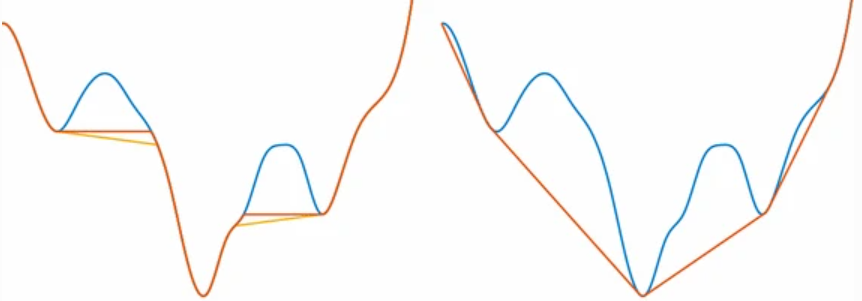
\includegraphics[scale=0.6]{figures/Einhuellende.png}
\end{figure}

Dieser klassisch relaxierte Weg wird hier nicht weiter diskutiert, sondern wir verweisen auf \cite{RelaxPaper} für mehr Details. Stattdessen werden wir den viel interessanteren und optimaleren Lösungsweg aus \cite{RelaxPaper} mithilfe von sogenannten Young-Maßen detailierter ausführen, die Informationen aus \cite{RelaxPaper} also präzesieren. Der Zusammenhang von Young-Maßen und Unterhalbstetigkeit/Konvexität wird später für die Theorie der Phasen-\\übergänge noch wichtig werden.\\

\textbf{Bemerkung:} Aus der gewohnten reellen Analysis heraus könnte hier durchaus \\(berechtigt) die Frage aufkommen, inwiefern eine konvexe Funktion nicht unterhalbstetig sein kann. Und tatsächlich ist die Implikation erst außerhalb des klassich reellen Kontextes falsch, wie die folgende Proposition zeigt:\\[0.5cm]
\pgfsetfillopacity{0.1}\colorbox{generalYellow}{\begin{minipage}{16cm}{\textcolor{black}{\pgfsetfillopacity{1}}{\label{prop3.11}}}
\textbf{Proposition 3.11 (Konvexität und Unterhalbstetigkeit):} Betrachte \((\mathbb{R}^n,\mathcal{T}_{ecl}), \, \mathcal{A} \subset \mathcal{T}_{sub}\) als nicht-leere konvexe Teilmenge von \(\mathbb{R}^n\) und ein Funktional \(\mathcal{F}:\mathcal{A} \to X\).\\
Wir unterscheiden:
\begin{enumerate}
    \item Ist \(X=\mathbb{R}\), so gilt: 
        \begin{equation}(\mathcal{F} \text{ ist konvex. } \Rightarrow \,\mathcal{F}\text{ ist unterhalbstetig.})\end{equation}
    \item Ist jedoch \(X=\overline{\mathbb{R}}\), so gilt: 
        \begin{equation}(\mathcal{F} \text{ ist konvex. } \nRightarrow \,\mathcal{F}\text{ ist unterhalbstetig.})\end{equation}
\end{enumerate}
\end{minipage}}\\

\textsc{Beweis:} Wir zeigen zunächst (1): \\
Dies ist ein Standardresultat aus der konvexen Analysis. Wir merken hier an, dass unter den Voraussetzungen \(\mathcal{F}\) sogar lokal (da auf einem Ball) Lipschitz ist mit Lipschitz Konstante \(L \approx 2M\), wobei \(M\) der größte Bildpunkt (hier ist wichtig, dass \(\mathcal{F} \neq \infty\) ist!) der Punkte der konvexen Hülle von \(\mathcal{A}\) unter \(\mathcal{F}\) ist (hier wird dann auch die Konvexität von \(\mathcal{F}\) wichtig, um von der Beschränktheit zu Lipschitz Stetigkeit zu gelangen). Damit ist \(\mathcal{F}\) stetig (da \(\mathcal{A}\) konvex ist, also \(conv(\mathcal{A})\) = \(\mathcal{A}\) gilt) und insbesondere unterhalbstetig.

Nun zu (2): Wir definieren die Funktion:
\begin{equation}
    F:\mathbb{R} \to \overline{\mathbb{R}},\,F(x):=\begin{cases}0, \,x > 0 \\+ \infty, \, x \leq 0 \end{cases}.
\end{equation}
Diese Funktion ist offensichtlich konvex, aber nicht unterhalbstetig.\QEDB

\subsection{Young-Maß-Relaxierung}{\label{subsec:relaxyoung}}
In \cite{RelaxPaper} haben wir das berühmte Bolza-Problem betrachtet, i.e.:
\begin{equation}{\label{eq3.34}}
    \mathcal{F}:W^{1,4}(]a,b[) \to \mathbb{R}_0^+,\,\mathcal{F}(w) := \int_{a}^b ((w')^2 - 1)^2 + w^4\,d\lambda^1(x),
\end{equation}
dessen vereinfachte Lösung die Sägezahnfunktionenfolge ist. Vereinfacht deshalb, da dieses Problem aufgrund der fehlenden Unterhalbstetigkeit keinen Minimierer besitzt. Vor allem für derartige Oszillation-Probleme bietet die Young-Maß-Theorie die ideale Lösung. Dazu definieren wir:\\[0.5cm]
\pgfsetfillopacity{0.1}\colorbox{generalYellow}{\begin{minipage}{16cm}{\textcolor{black}{\pgfsetfillopacity{1}}{\label{def3.12}}}
\textbf{Definition 3.12 (Young-Maße):} Betrachte ein nicht-negatives Maß \(\vartheta \in \mathcal{M}(A \times \mathbb{R}^N), \, N \in \mathbb{N}\) mit A offen in \(\mathbb{R}^n, \, n \in \mathbb{N}\). Wir nennen \(\vartheta\) ein Young-Maß \(: \Leftrightarrow\)
\begin{equation}
    \pi_A \# \vartheta(B \times \mathbb{R}^N) = \lambda^n(B)
\end{equation}
für alle Borelmengen B auf A. Die zugehörige Menge bezeichnen wir mit \(\Y\).
\end{minipage}}

Im Folgenden topologisieren wir \(\Y\), indem wir den Raum mit der \\Einschränkungstopologie (Englisch: Narrow Topology) bezüglich \(\mathcal{C}_m(A,\mathbb{R}^N), \, N \in \mathbb{N}\) ausstatten. Hierbei bezeichnet \(\mathcal{C}_m(A,\mathbb{R}^N)\) den Raum aller Caratheodory-Integranden. Die Einschränkungstopologie entspricht der Initialtopologie für Caratheodory-Integranden.\\
Wir erhalten die dementsprechende eingeschränkte Konvergenz definiert durch:
\begin{equation}
    \vartheta_k \stackrel{nar}{\rightharpoonup} \vartheta :\Leftrightarrow \lim_{k \to \infty} \int_{A \times \mathbb{R}^N} \psi (x,y) \, d\vartheta_k (x,y) = \int_{A \times \mathbb{R}^N} \psi(x,y) \, d\vartheta(x,y)
\end{equation}
für alle \(k,N \in \mathbb{N}, \, \psi \in \mathcal{C}_m(A,\mathbb{R}^N)\).\\

Um Relaxierungsprobleme mithilfe eines Young-Maßes lösen zu können - und auch, um die Intuition dahinter verstehen zu können - müssen wir nun etwas Wahrscheinlichkeitstheorie betreiben. Die Beweise sind teils sehr aufwändig und würden zu weit von unserem eigentlichen Fokus dieser Arbeit wegführen, weshalb wir für die Beweise auf die jeweilige Quelle verweisen. Nun existiert zu jedem Young-Maß eine ganze Familie an Wahrscheinlichkeitsmaßen, i.e. es gilt:
\begin{equation}{\label{eq3.37}}
    \Y \ni \vartheta = (\vartheta_x)_{x \in A} \otimes \lambda^n.
\end{equation}
Die Messbarkeit bezüglich dieses Maßes ist dann unter der zugehörigen Produkt-\(\sigma\)-Algebra zu verstehen. Warum \eqref{eq3.37} überhaupt so existiert, beantwortet folgender Satz:\\[0.5cm]
\pgfsetfillopacity{0.1}\colorbox{generalYellow}{\begin{minipage}{16cm}{\textcolor{black}{\pgfsetfillopacity{1}}{\label{theo3.13}}}
\textbf{Satz 3.13 (Fubini für Wahrscheinlichkeitsmaße, \cite{AttouchCalcVar}[Theorem 4.2.4.]):} Es sei \(\rho = \pi_A \vartheta\). Dann existiert eine Familie an Wahrscheinlichkeitsmaßen \((\vartheta_x)_{x \in A}\) in \(\mathbb{R}^N, \, N \in \mathbb{N}, \, \rho-\)f.ü., sodass für \(f \in \mathcal{C}_0 (A \times \mathbb{R}^N)\) gilt:
\begin{enumerate}
    \item \(x \mapsto \int_{\mathbb{R}^N} f(x,y) \, d\vartheta_x(y)\) ist \(\rho\)-messbar.
    \item \(\int_{A \times \mathbb{R}^N} f(x,y) \, d\vartheta(x,y) = \int_A (\int_{\mathbb{R}^N} f(x,y) \, d\vartheta_x(y))\, d\rho(x)\).
\end{enumerate}
\end{minipage}}

Wir widmen uns nun der Existenz- und Wohldefiniertheitstheorie von Young-Maßen in Relaxierungsproblemen zu. Im Anschluss werden wir das Verhalten gegenüber Oszillationen beschreiben und im Zuge dessen dann auch präsentieren, wie man konkrete Anwendungsbeispiele, wie das Bolza-Problem, dann tatsächlich auch löst mithilfe der Young-Theorie. Zunächst sei hier eine sehr wichtige Eigenschaft der Young-Maße aufgeführt:\\[0.5cm]
\pgfsetfillopacity{0.1}\colorbox{generalYellow}{\begin{minipage}{16cm}{\textcolor{black}{\pgfsetfillopacity{1}}{\label{lem3.14}}}
\textbf{Lemma 3.14 (Unterhalbstetigkeit von Young-Maßen I, \cite{AttouchCalcVar}[Proposition 4.3.3.]):} Seien \(k,n,N \in \mathbb{N}, \, \) \(\Y \supset \{\vartheta_k\} \stackrel{nar}{\rightharpoonup} \vartheta \in \Y, \, \psi : A \times \mathbb{R}^N \to [0,\infty]\) eine \(\mathcal{M}^n(\mathbb{R}^n) \otimes \mathcal{B}(\mathbb{R}^N)\)-messbare Funktion, die für \(\lambda^n\)-f.a. x in A unterhalbstetig ist. Dann gilt:
\begin{equation}
    \int_{A \times \mathbb{R}^N} \psi(x,y) \, d\vartheta(x,y) \leq \liminf_{k \to \infty} \int_{A \times \mathbb{R}^N} \psi(x,y) \, d\vartheta_k(x,y). 
\end{equation}
\end{minipage}}

Die Annahme für \(\psi\) war hierbei allerdings viel zu restriktiv. Stattdessen werden wir das Resultat nun auf einen signierten Fall erweitern. Wir brauchen zwar eine Beschränkung nach unten, es wird sich aber herausstellen, dass es ausreicht, falls der negative Anteil von \(\psi\) eine vernachlässigbare Wahrscheinlichkeitsmasse zum Erwartungswert beiträgt. Dies führt auf eine Kompaktheitsbedingung, die man auch gleichmäßige Integrierbarkeit nennt. Der Beweis greift auf das Resultat [\ref{lem3.14}, Lemma 3.14] dann zurück und das Theorem liest sich wie folgt:\\[0.5cm]
\pgfsetfillopacity{0.1}\colorbox{generalYellow}{\begin{minipage}{16cm}{\textcolor{black}{\pgfsetfillopacity{1}}{\label{theo3.15}}}
\textbf{Satz 3.15 (Unterhalbstetigkeit von Young-Maßen II, \cite{AttouchCalcVar}[Proposition 4.3.4.]):} Seien \(\Y \supset \{\vartheta_k\} \stackrel{nar}{\rightharpoonup} \vartheta \in \Y, \, \psi : A \times \mathbb{R}^N \to \mathbb{R}\) eine \(\mathcal{M}^n(\mathbb{R}^n) \otimes \mathcal{B}(\mathbb{R}^N)\)-messbare Funktion, die für \(\lambda^n\)-f.a. x in A unterhalbstetig ist. Ist \(x \mapsto \psi(x,y_k))_{-}\) gleichmäßig integrierbar, i.e. es gilt:
\begin{equation}{\label{eq3.39}}
    \lim_{Y \to \infty} \mathbb{E}[|y_k| \chi_{\{|y_k| \geq Y\}}] = 0,
\end{equation}
dann gilt:
\begin{equation}
    \int_{A \times \mathbb{R}^N} \psi(x,y) \, d\vartheta(x,y) \leq \liminf_{k \to \infty} \int_A \psi(x,y_k) \, d\lambda^n(x). 
\end{equation}
\end{minipage}}

\textbf{Bemerkung:} Der Limes in \eqref{eq3.39} existiert in dem vorliegendem Fall dank einer majorisierten Konvergenz. Es muss insbesondere die betrachtete Zufallsvariable (hier \(y_k\)) in \(L^1\) liegen.\\

In der Anwendung sind meistens bessere Bedingungen gegeben. Erweitert man Unterhalbstetigkeit auf Stetigkeit und die gleichmäßige Integrierbarkeit auf ganz \(\psi\), erhält man auch ein viel stärkeres Resultat:\\[0.5cm]
\pgfsetfillopacity{0.1}\colorbox{generalYellow}{\begin{minipage}{16cm}{\textcolor{black}{\pgfsetfillopacity{1}}{\label{kor3.16}}}
\textbf{Korollar 3.16 (Unterhalbstetigkeit von Young-Maßen III, \cite{AttouchCalcVar}[Theorem 4.3.3.]):} Seien \(\Y \supset \{\vartheta_k\} \stackrel{nar}{\rightharpoonup} \vartheta \in \Y, \, \psi : A \times \mathbb{R}^N \to \mathbb{R}\) eine \(\mathcal{M}^n(\mathbb{R}^n) \otimes \mathcal{B}(\mathbb{R}^N)\)-messbare Funktion, die für \(\lambda^n\)-f.a. x in A \textbf{stetig} ist. Ist \(x \mapsto \psi(x,y_k)\) gleichmäßig integrierbar, dann gilt:
\begin{equation}
    \int_{A \times \mathbb{R}^N} \psi(x,y) \, d\vartheta(x,y) = \lim_{k \to \infty} \int_A \psi(x,y_k) \, d\lambda^n(x). 
\end{equation}
\end{minipage}}

\textsc{Beweis:} Folgt direkt aus einer Anwendung von [\ref{theo3.15}, Satz 3.15] auf den Positiv- und Negativteil von \(\psi\).\QEDB

Nachdem wir jetzt die wichtigsten Eigenschaften für Young-Maße gesehen haben, stellt sich gerade für die Anwendung später natürlich noch die Frage, wann und wie man solche Maße im Allgemeinen überhaupt erzeugt (bzw. erzeugen kann). Das folgende Fundamentaltheorem wurde in seiner Grundidee von L. Young selbst 1942 in \cite{young1942generalized} und \cite{youngII1942generalized} erarbeitet und später von J. Ball 1988 in \cite{ball2005version} für die Variationsrechnung nützlich gemacht. Wir benutzen an dieser Stelle die Notation von F. Bethuel, G. Huisken, S. Müller und K. Steffen aus \cite{bethuel1999variational}[Theorem 3.1 (Fundamental theorem on Young measures)]:\\[0.5cm]
\pgfsetfillopacity{0.1}\colorbox{generalYellow}{\begin{minipage}{16cm}{\textcolor{black}{\pgfsetfillopacity{1}}{\label{theo3.17}}}
\textbf{Satz 3.17 (Fundamentaltheorem für Young-Maße):} Sei \(E \subset \mathcal{M}^n(\mathbb{R}^n)\) mit endlichem Lebesgue-Maß, \(w_k : E \to \mathbb{R}^N\) \(\mathcal{M}^n(\mathbb{R}^n)\)-messbar. Dann existiert eine Teilfolge \(w_{k_l}\), die \(\vartheta \in \mathcal{Y}(E,\mathbb{R}^N)\) erzeugt, i.e. eine Abbildung \(\vartheta \in L^{\infty}_{w^*}(E,\mathcal{M}(\mathbb{R}^N))\). Das erzeugte Young-Maß \(\vartheta\) besitzt dann folgende Eigenschaften:
\begin{enumerate}
    \item \((\vartheta_x \geq 0 \, \, \land \, \, ||\vartheta_x||_{\mathcal{M}(\mathbb{R}^N)} = \int_{\mathbb{R}^N} d\vartheta_x \leq 1) \text{ f. }\lambda^n-\text{f.a. }x\),
    \item \(\forall f \in C_0(\mathbb{R}^N) \, : \, f(w_{k_l}) \stackrel{*}{\rightharpoonup} <\vartheta_x,f> \stackrel{Riesz}{=} \int_{\mathbb{R}^N} fd \vartheta_x\) in \(L^{\infty}(E)\),
    \item Ist \(K\) eine kompakte Menge im \(\mathbb{R}^N\), dann gilt: \((d_{\mathbb{R}^n} (w_{k_l}, K) \stackrel{\vartheta}{\to} 0 \, \Rightarrow \, supp \, \vartheta_x \subset K\)),
    \item (\(\lim_{C \to \infty} \sup_{l \in \mathbb{N}} \lambda^n(\{|w_{k_l}| \geq C\}) = 0 \, \Leftrightarrow \, ||\vartheta_x||_{\mathcal{M}(\mathbb{R}^N)} = 1 \text{ f. }\lambda^n-\text{f.a. }x\)),
    \item Ist \(||\vartheta_x||_{\mathcal{M}(\mathbb{R}^N)} = 1\), dann gilt \(\Leftrightarrow\) in (3), sowie mit \(B \subset \mathcal{M}^n(E), \text{ und} f(w_{k_l}) \in \overline{\mathcal{K}}_w(L^1(B))\):
    \begin{equation}
        f(w_{k_l}) \rightharpoonup <\vartheta_x,f> \text{ in }L^1(B).
    \end{equation}
\end{enumerate}
\end{minipage}}

\textbf{Bemerkung:} (2) ist wohldefiniert, da nach Riesz
\begin{equation}
    \mathcal{M}(\mathbb{R}^N) \simeq (C_0(\mathbb{R}^N))^*
\end{equation}
gilt, siehe [\ref{theo2.6}, Satz 2.6].\\

Wir werden nun auf das sehr gute Verhalten von Young-Maßen gegenüber Oszillationen eingehen und folgen dabei \cite{AttouchCalcVar}[Seite 146]. Intuitiv gesprochen ist die Young-Theorie für Probleme wie das Bolza-Problem \eqref{eq3.34} die optimale Lösung, da Young-Maße für f.a. \(x \in A\) angeben, wie sich die gleichmäßig verteilte Wahrscheinlichkeitsmasse von \(y_k\) verhalten muss. Oft ist die Lösung deshalb dann eine Kombination an Dirac-Maßen. Diese Behauptung wollen wir nun mathematisch beweisen:\\
Zunächst wenden wir [\ref{theo3.13}, Satz 3.13] mit 
\begin{equation}
    (x,y) \mapsto \chi_{B_r(x_0) \times \Omega} (x,y) \, \, \forall x_0 \in A, \, r > 0, \, \Omega \subset \mathcal{T}_{ecl,sub}
\end{equation}
an und erhalten:
\begin{equation}
    \vartheta(B_r(x_0) \times \Omega) = \int_{A \times \mathbb{R}^N} \chi_{B_r(x_0) \times \Omega} (x,y) \,d\vartheta(y) = \int_{B_r(x_0)} \vartheta_x(\Omega) \,d\lambda^n(x).
\end{equation}
Jetzt benutzen wir [\ref{lem2.3}, Lemma 2.3] und es folgt:
\begin{equation}
    \vartheta_{x_0} (\Omega) = \lim_{r \to 0} \frac{1}{\lambda^n(B_r(x_0))} \vartheta(B_r(x_0) \times \Omega) \text{ f.f.a. }x_0 \in A.
\end{equation}
Die Größe der Nullmenge, auf der die Aussage nicht gilt, korrespondiert dabei natürlich mit dem Komplement der Menge der Lebesgue-Punkte. Wähle nun r, sodass
\begin{equation}
    \vartheta(\partial(B_r(x_0) \times \Omega)) = 0
\end{equation}
gilt. Die Existenz dieser Wahl ist sichergestellt, da für nicht-negatives \(\nu \in \mathcal{M}(A)\) eine Teilindexierung für disjunkte Borelmengen in A höchstens abzählbar nicht verschwindet bezüglich \(\nu\). Da \(\vartheta_k\) eingeschränkt konvergiert, gilt insbesondere \(\vartheta_k \rightharpoonup \vartheta\). Damit folgt mit dem Kompaktheitssatz von Prokhorov (siehe [\ref{korA.5}, Anhang A.5]):
\begin{equation}
    \vartheta(B_r(x_0) \times \Omega) = \lim_{k \to \infty} \lambda^n(\{x \in B_r(x_0) \, | \, y_k(x) \in \Omega\})
\end{equation}
und damit insgesamt die Behauptung:
\begin{equation}
    \vartheta_{x_0}(\Omega) = \lim_{r \to 0} \lim_{k \to \infty} \frac{\lambda^n(\{x \in B_r(x_0) \, | \, y_k(x) \in \Omega\})}{\lambda^n(B_r(x_0))}.
\end{equation}
Die Wohldefiniertheit dieses Ausdruckes ist durch den Satz von Radon-Nikodym \\sichergestellt.
%%%%%%%%%%%%%%%%%%%%%%%%%%%%%%%%%%%%%%%%%%%%%%%%%%%%%%%%%%%%%%%%%%%%%%%%%%%%%%%%%%%%%%%%%%%%%%%%%%%%%%%%%%%%%
\section{Moreau-Yosida Approximation}{\label{sec:moryos}}
In \ref{sec:gammaprop} haben wir ein Existenzresultat für Integralfunktionale kennengelernt. Wir werden nun ein zweites kennenlernen, diesmal für nicht notwendigerweise Integralfunktionale, sondern Funktionale, die auf einem allgemeinen metrischen Raum definiert sind. Im idealen Rahmen wird sich herausstellen, dass sich auch eine Verbindung zur Relaxierung finden lässt. Diese Vorgedanken führen auf die sogenannte Moreau-Yosida Approximation. Wir werden in diesem Unterkapitel von Beweisen absehen (sie sind natürlich in der angegebenen Quelle zu finden), da die Moreau-Yosida Approximation nur indirekt Anwendung für den Kern dieser Arbeit findet.\\[0.5cm]
\pgfsetfillopacity{0.1}\colorbox{generalYellow}{\begin{minipage}{16cm}{\textcolor{black}{\pgfsetfillopacity{1}}{\label{def3.18}}}
\textbf{Definition 3.18 (Moreau-Yosida Approximation, \cite{MasoGamma}[Definition 9.8.]):} Sei \((\mathcal{X},d_{\mathcal{X}})\) ein metrischer Raum, \(\alpha > 0, \, \tau > 0\). Wir definieren für das Funktional \(\mathcal{F} : \mathcal{X} \to \overline{\mathbb{R}}\) die Moreau-Yosida Approximation der Ordnung \(\alpha\) und des Indexes \(\tau\) durch:
\begin{equation}
    \mathcal{F}^{\alpha,\tau} : \mathcal{X} \to \overline{\mathbb{R}}, \, \mathcal{F}^{\alpha, \tau}(x) := \inf_{y \in \mathcal{X}} \{\mathcal{F}(y) + \tau d(x,y)^{\alpha}\} \, \, \forall x \in \mathcal{X}.
\end{equation}
\end{minipage}}\\

Schnell verfestigt sich der Eindruck, dass diese Approximation etwas an die Relaxierung erinnert und wie anfangs bereits erwähnt, ist das tatsächlich der Fall:\\[0.5cm]
\pgfsetfillopacity{0.1}\colorbox{generalYellow}{\begin{minipage}{16cm}{\textcolor{black}{\pgfsetfillopacity{1}}{\label{prop3.19}}}
\textbf{Proposition 3.19 (Moreau-Yosida Approximation und Relaxierung, \cite{MasoGamma}[Remark 9.1.]):} Sei \((\mathcal{X},d_{\mathcal{X}})\) ein metrischer Raum, \(\alpha > 0, \, \tau > 0, \, \mathcal{F} : \mathcal{X} \to [0,\infty]\). Dann gilt:
\begin{equation}
    sc^- \mathcal{F} = \sup_{\tau > 0} \mathcal{F}^{\alpha, \tau}.
\end{equation}
\end{minipage}}

Eine Beziehung zur \(\Gamma\)-Konvergenz lässt sich natürlich auch herstellen:\\[0.5cm]
\pgfsetfillopacity{0.1}\colorbox{generalYellow}{\begin{minipage}{16cm}{\textcolor{black}{\pgfsetfillopacity{1}}{\label{theo3.20}}}
\textbf{Satz 3.20 (Moreau-Yosida Approximation und \(\Gamma\)-Konvergenz, \cite{MasoGamma}[Theorem 9.7.]):} Sei \((\mathcal{X},d_{\mathcal{X}})\) ein metrischer Raum, \(\Phi\) wie in [\ref{theo3.9}, Satz 3.9], \(\mathcal{F}_h, \mathcal{F} : \mathcal{X} \to [0,\infty], \, \mathcal{F}\) unterhalbstetig. Angenommen, es existiert \(\kappa > 0\), sodass für alle \(x \in \mathcal{X}\)
\begin{equation}
    \mathcal{G}_h(y) := \mathcal{F}_h(y) + \kappa \Phi(d(x,y))
\end{equation}
gleichgradig koerziv auf \(\mathcal{X}\) ist. Sei \(\{\tau_j\}_{j \in \mathbb{N}} \to \infty\), sodass \(\tau_j \geq \kappa\). Dann gilt:
\begin{equation}
    (\mathcal{F}_h \stackrel{\Gamma}{\to} \mathcal{F} \, \Leftrightarrow \, \forall j \in \mathbb{N} \, \forall x \in \mathcal{X} \, : \, \inf_{y \in \mathcal{X}} \{\mathcal{F}(y) + \tau_j \Phi(d(x,y))\} = \lim_{h \to \infty} \inf_{y \in \mathcal{X}} \{\mathcal{F}_h(y) + \tau_j \Phi(d(x,y))\}).
\end{equation}
\end{minipage}}
Für das Funktional \(\mathcal{F}\) sehen wir direkt aus der Definition des Infimums, dass falls \(\alpha \in ]0,1]\) ist, Folgendes gilt:
\begin{equation}
    \mathcal{F}^{\alpha, \tau} \leq \mathcal{F}.
\end{equation}
In dieser Situation fühlt man sich stark an die Hölder-Stetigkeit erinnert und genau das kann man auch zeigen:\\[0.5cm]
\pgfsetfillopacity{0.1}\colorbox{generalYellow}{\begin{minipage}{16cm}{\textcolor{black}{\pgfsetfillopacity{1}}{\label{theo3.21}}}
\textbf{Satz 3.21 (Hölder-Stetigkeit der Moreau-Yosida Approximation, \cite{MasoGamma}[Theorem 9.13.]):} Sei \((\mathcal{X},d_{\mathcal{X}})\) ein metrischer Raum, \(\alpha \in ]0,1], \, \tau > 0, \, \mathcal{G} : X \to \overline{\mathbb{R}}\). Dann ist \(\mathcal{F}^{\alpha, \tau}\) das größte \(\mathcal{G}\), welches folgende Eigenschaften trägt:
\begin{enumerate}
    \item \(\mathcal{G} \leq \mathcal{F}\),
    \item \(\mathcal{G} \in \mathcal{C}^{0,\alpha}(X,\overline{\mathbb{R}}), \, C_{hld} = \tau\).
\end{enumerate}
\end{minipage}}

Generell ist Lipschitz-Regularität zu erwarten:\\[0.5cm]
\pgfsetfillopacity{0.1}\colorbox{generalYellow}{\begin{minipage}{16cm}{\textcolor{black}{\pgfsetfillopacity{1}}{\label{theo3.22}}}
\textbf{Satz 3.22 (Lipschitz-Stetigkeit der Moreau-Yosida Approximation, \cite{MasoGamma}[Theorem 9.15.]):} Sei \((\mathcal{X},d_{\mathcal{X}})\) ein metrischer Raum, \(\alpha \geq 1, \, \tau > 0, \, C_1 \geq 0, \, r > 0, \, \mathcal{F} : \mathcal{X} \to [0,\infty]\). Dann gilt:
\begin{equation}
    (\mathcal{F}^{\alpha, \tau} \leq C_1 \, \Rightarrow \, \exists C_{lip} = C_{lip} (\alpha,\tau,C_1,r) : \, \mathcal{F}^{\alpha,\tau} \in Lip_{loc}(\mathcal{X},[0,\infty])).
\end{equation}
\end{minipage}}

Wir werden nun das zu Beginn angekündigte Existenztheorem für die \(\Gamma\)-Konvergenz präsentieren. Um die Äquivalenz zu gewährleisten, benötigen wir erneut eine Kompaktheitseigenschaft. Für (seperable) metrische Räume reicht hierfür eine Koerzivitätseigenschaft und das Theorem lautet dann wie folgt:\\[0.5cm]
\pgfsetfillopacity{0.1}\colorbox{generalYellow}{\begin{minipage}{16cm}{\textcolor{black}{\pgfsetfillopacity{1}}{\label{theo3.23}}}
\textbf{Satz 3.23 (\(\Gamma\)-Konvergenz Existenztheorem, metrische Version, \cite{MasoGamma}[Theorem 9.16.]):} Sei \((\mathcal{X},d_{\mathcal{X}})\) ein (seperabler) metrischer Raum (falls nicht seperabel, so betrachte den Raum selber), \(\alpha > 0, \, \mathcal{F}, \mathcal{F}_h : \mathcal{X} \to [0,\infty], \\ \mathcal{F}_h \text{ gleichgradig koerziv}, \, \mathcal{F} \text{ unterhalbstetig}\). Betrachte eine dichte Teilmenge \(Y\) von \(X\) und \(\mathbb{R}^+ \supset \{\tau_j\} \to \infty\). Dann gilt:
\begin{enumerate}
    \item \(\GaLim \mathcal{F}_h = \mathcal{F} \, \Leftrightarrow\)
    \item \(\mathcal{F}^{\alpha, \tau_j} = \lim_{h \to \infty} \mathcal{F}_h^{\alpha, \tau_j}\) auf \(Y\).
\end{enumerate}
\end{minipage}}
%%%%%%%%%%%%%%%%%%%%%%%%%%%%%%%%%%%%%%%%%%%%%%%%%%%%%%%%%%%%%%%%%%%%%%%%%%%%%%%%%%%%%%%%%%%%%%%%
\section[Topologische Betrachtung der Gamma-Konvergenz]{Topologische Betrachtung der \(\Gamma\)-Konvergenz}{\label{sec:gammatopo}}
Die direkte Methode [\ref{theo2.8}, Satz 2.8] und das bisher gesehene grundlegende Verhalten der \(\Gamma\)-Konvergenz haben uns gezeigt, dass \(\Gamma\)-Konvergenz und Unterhalbstetigkeit sehr stark zusammenhängen. Wenn wir Konvergenzbegriffe betrachten in der Analysis, stellen wir uns immer als eine der ersten Fragen: Bezüglich welcher Topologie? Wir werden deshalb in diesem Unterkapitel eine passende Topologie \(\mathcal{T}\) für den Raum der unterhalbstetigen Funktionen über dem (T2)-Raum \((X,\mathcal{T}_X)\) ansehen. Diesen Raum werden wir mit \(\mathcal{S}(X)\) notieren im Folgenden. Wir werden dabei die Äquivalenz von \(\Gamma\)-Konvergenz und Konvergenz bezüglich \(\mathcal{T}_{X,Sub}\) sehen (Klassisch lernt man: die notwendige Bedingung ist allgemein erfüllt; für die hinreichende Bedingung muss \(X\) zusätzlich lokal kompakt sein bzw. das 1.AA erfüllen; wir werden sehen, dass wir hier mit weniger algebraischer Struktur an unser Ziel kommen werden.). Da wir im Folgenden (fast immer) nur die Relativtopologie und nicht die Topologie von \(X\) benötigen werden, notieren wir - auch zur besseren Lesbarkeit - im Folgenden \(\mathcal{T}:=\mathcal{T}_{X,Sub}\). Es sei hier noch angemerkt, dass natürlich Funktionale \(\mathcal{F} \in \mathcal{S}(X)\) gemeint sind, die in \(\overline{\mathbb{R}}\) abbilden, wie gewohnt. Betrachte dann für \(\Omega \subset X\):
\begin{equation}
    \mathcal{I}:\mathcal{S}(X) \to \overline{\mathbb{R}}, \, \mathcal{I}(\Omega,\mathcal{F}) := \inf_{x \in \Omega} \mathcal{F}(x),
\end{equation}
wobei wir \(\inf \emptyset := \infty\) setzen, um die Wohldefiniertheit zu gewähren. Im Folgenden sind wir dann interessiert an:\\[0.5cm]
\pgfsetfillopacity{0.1}\colorbox{generalYellow}{\begin{minipage}{16cm}{\textcolor{black}{\pgfsetfillopacity{1}}{\label{def3.24}}}
\textbf{Definition 3.24 \cite{MasoGamma}[Definition 10.1]:} Sei \(U \subset X\) offen (bezüglich \(\mathcal{T}\)), \(K \subset X\) kompakt. In natürlicher Weise setzen wir:
\begin{enumerate}
    \item \(\mathcal{T}^+\) für die schwächste Topologie auf \(\mathcal{S}(X)\), für die \(\mathcal{I}(U)\) oberhalbstetig sind,
    \item \(\mathcal{T}^-\) für die schwächste Topologie auf \(\mathcal{S}(X)\), für die \(\mathcal{I}(K)\) unterhalbstetig sind und
    \item in Folge dessen notiert \(\mathcal{T}\) dann die schwächste Topologie auf \(\mathcal{S}(X)\), die stärker als \(\mathcal{T}^+\) und \(\mathcal{T}^-\) ist.
\end{enumerate}
\end{minipage}}

\textbf{Bemerkung:} Man könnte sich nun in (2) fragen, warum wir hier eine kompakte Teilmenge fordern. Der Grund dafür ist (wie wir gleich sehen werden), dass \(X\) eine Kohärenz-Eigenschaft nicht erfüllt, die benötigt wird.\\

Die analytische Betrachtung der Äquivalenz aus der Motivation wird uns zu folgenden zwei Sätzen führen:\\[0.5cm]
\pgfsetfillopacity{0.1}\colorbox{generalYellow}{\begin{minipage}{16cm}{\textcolor{black}{\pgfsetfillopacity{1}}{\label{theo3.25}}}
\textbf{Satz 3.25 \cite{MasoGamma}[Theorem 10.6]:} \((\mathcal{S}(X),\mathcal{T}^+), \, (\mathcal{S}(X),\mathcal{T}^-), \, (\mathcal{S}(X),\mathcal{T})\) sind kompakt.
\end{minipage}}
\newpage
\pgfsetfillopacity{0.1}\colorbox{generalYellow}{\begin{minipage}{16cm}{\textcolor{black}{\pgfsetfillopacity{1}}{\label{theo3.26}}}
\textbf{Satz 3.26 (Topologische direkte Methode der \(\Gamma\)-Konvergenz, \cite{MasoGamma}[Corollary 10.10]):} Sei \(\{\mathcal{F}_h\}_{h \in \mathbb{N}} \subset \mathcal{S}(X), \, \mathcal{F} \in \mathcal{S}(X)\), dann gilt:
\begin{equation}{\label{eq3.57}}
\begin{array}{l}
    \mathcal{F}_h \stackrel{\mathcal{T}}{\to} \mathcal{F} \, \Leftrightarrow \\
    \Gamma-\limsup_{h \to \infty} \mathcal{F}_h \leq \mathcal{F}(x) \leq \sup_{U \in \mathcal{N}(x)} \inf_{K \in \mathcal{K}(U)} \liminf_{h \to \infty} \inf_{y \in K} \mathcal{F}_h(y).
\end{array}
\end{equation}
\end{minipage}}

\eqref{eq3.57} sieht verdächtig nach unserem angestrebten Äquivalenzresultat aus. Der einzige Unterschied ist, dass wir uns für den \(\Gamma\)-Liminf auf einer kompakten Teilmenge bewegen. Folgendes Beispiel zeigt, dass die gegebene algebraische Struktur unser Zielresultat auch noch nicht zulässt:\\
Betrachte \(X\) als den Hilbertraum \((\mathcal{H},\mathcal{T}_w)\) mit \(dim(\mathcal{H}) = \infty, \, \mathcal{T}_w\) der schwachen Topologie auf \(\mathcal{H}\). Für eine orthonormale Folge \(\{e_h\}\) in \(\mathcal{H}\) betrachte:
\begin{equation}
    \mathcal{F}_h(x) := ||1 - \frac{1}{h} <x,e_h>_{\mathcal{H}}||_{Fr}.
\end{equation}
Zwar \(\Gamma\)-konvergiert \(\mathcal{F}_h\) gegen 0 in \(\mathcal{H}\), jedoch gilt:
\begin{equation}
    \mathcal{F}_h \stackrel{\mathcal{T}}{\to} \mathcal{F},
\end{equation}
wobei \(\mathcal{F} \in \mathcal{S}(X)\) mit \(\mathcal{F} \in [0,1]\). Für einen Beweis verweisen wir auf \cite{MasoGamma}[Example 10.11].\\

Es stellt sich heraus, dass die fehlende Struktur topologische Kohärenz bezüglich kompakten (T2)-Unterräumen ist. In der Topologie spricht man von einem Kelley-Raum (Englisch: k-space). Da der Beweis sehr technisch ist und wenig neue Intuition ergänzend zu [\ref{theo3.26}, Satz 3.26] liefert, verweisen wir für den Beweis auf \cite{MasoGamma}[Lemma 10.16]. Wir bemerken hier noch kurz, dass die Intuition dadurch nicht zerstört wird, da jeder (T2)-Raum, der lokal kompakt ist bzw. das 1.AA erfüllt, ein Kelley-Raum ist. Bevor wir uns nun den Beweisen widmen, benötigen wir noch etwas Vorarbeit, die uns die Konvergenz bezüglich der drei Topologien \(\mathcal{T}, \, \mathcal{T}^+, \, \mathcal{T}^-\) charakterisiert:\\[0.5cm]
\pgfsetfillopacity{0.1}\colorbox{generalYellow}{\begin{minipage}{16cm}{\textcolor{black}{\pgfsetfillopacity{1}}{\label{lem3.27}}}
\textbf{Lemma 3.27 \cite{MasoGamma}[Proposition 10.3]:} Sei \(\{\mathcal{F}_h\}_{h \in \mathbb{N}}\) eine Folge in \(\mathcal{S}(X)\), \(U \subset X\) eine (bezüglich \(\mathcal{T}\)) offene Teilmenge, \(K \subseteq X\) eine kompakte Teilmenge. Diese Folge konvergiert gegen \(\mathcal{F} \in \mathcal{S}(X)\) bezüglich der Topologie, falls Infimum/Supremum in \(U\) bzw. \(K\) existieren und...
\begin{enumerate}
    \item \(\mathcal{T}^+ \, \Leftrightarrow \, \inf_{x \in U} \mathcal{F}(x) \geq \limsup_{h \to \infty} \inf_{x \in U} \mathcal{F}_h(x)\);
    \item \(\mathcal{T}^- \, \Leftrightarrow \, \inf_{x \in K} \mathcal{F}(x) \leq \liminf_{h \to \infty} \inf_{x \in U} \mathcal{F}_h(x)\);
    \item \(\mathcal{T} \, \Leftrightarrow \,\)(1) und (2) erfüllt sind.
\end{enumerate}
\end{minipage}}

\textsc{Beweis:} Zunächst erinnern wir daran, dass \((\mathbb{R},\mathcal{T}_{ecl})\) folgende Subbasis besitzt:
\begin{equation}
    \mathcal{S} := \mathcal{S}^+ \cup \mathcal{S}^- := \{x \in \mathbb{R} \, | \, x > y, \, y \in \mathbb{R}\} \, \cup \, \{x \in \mathbb{R} \, | \, x < y, \, y \in \mathbb{R}\}. 
\end{equation}
Damit ist klar, dass Folgendes gilt:
\begin{itemize}
    \item Die Subbasis von \(\mathcal{T}^+\) ist gegeben durch: \(\mathcal{S}_{\mathcal{T}}^+ := \bigcup_{i \in I}\{\mathcal{F} \in \mathcal{S}(X) \, | \, \mathcal{I}(U_i,\mathcal{F}) < t_i\}\) mit \(t_i\) aus einer dichten Teilmenge von \(\mathbb{R}\).
    \item Die Subbasis von \(\mathcal{T}^-\) ist gegeben durch: \(\mathcal{S}_{\mathcal{T}}^- := \bigcup_{j \in J} \{\mathcal{F} \in \mathcal{S}(X) \, | \, \mathcal{I}(K_j,\mathcal{F}) > s_j\}\) mit \(s\) aus einer dichten Teilmenge von \(\mathbb{R}\).
    \item Die Subbasis von \(\mathcal{T}\) ist dann gegeben durch: \(S_{\mathcal{T}} := \mathcal{S}_{\mathcal{T}}^+ \, \cup \, \mathcal{S}_{\mathcal{T}}^-\).
\end{itemize}
Wir halten noch fest, dass man Limsup und Liminf auch wie folgt charakterisieren kann:
\begin{itemize}
    \item \(\liminf_{h \to \infty} \mathcal{F}_h = \bigcup_{h=1}^{\infty}(\bigcap_{m=h}^{\infty} \mathcal{F}_m)\),
    \item \(\limsup_{h \to \infty} \mathcal{F}_h = \bigcap_{h=1}^{\infty}(\bigcup_{m=h}^{\infty} \mathcal{F}_m)\).
\end{itemize}
Nach der grundlegenden Definition bilden endliche Schnitte an Mengen aus der Subbasis eine Basis für eine Topologie. Unmittelbar aus der Definition der jeweils betrachteten Topologien und der Konvergenz in topologischen Räumen folgt dann sofort die Behauptung. \QEDB

Wir befinden uns nun in der Situation, die beiden Resultate [\ref{theo3.25}, Satz 3.25] und [\ref{theo3.26}, Satz 3.26] beweisen zu können:\\

\textsc{Beweis von Satz 3.25:} Nach [\ref{lem3.27}, Lemma 3.27] wissen wir, wie die Subbasen von \(\mathcal{T}, \, \mathcal{T}^+, \, \mathcal{T}^-\) aussehen. Das Subbasis-Theorem von Alexander (Achtung, benutzt in essentieller Weise das Lemma von Zorn, welches logisch äquivalent zum Auswahlaxiom ist!) sichert uns dann, dass wir die Kompaktheit nur für die jeweilige Subbasis nachweisen müssen. Nun sind \(\mathcal{T}^+\) und \(\mathcal{T}^-\) nach Definition schwächer als \(\mathcal{T}\). Es reicht also zu zeigen, dass \((\mathcal{S}(X),\mathcal{T})\) kompakt bezüglich seiner Subbasis ist. Betrachte also:
\begin{equation}
    G: X \to \overline{\mathbb{R}}, \, G(x) := \sup \{t_i \, | \, i \in I, \, x \in U_i\},
\end{equation}
wobei \(\sup \emptyset = - \infty\). Diese Funktion ist nach Definition unterhalbstetig auf \(X\). Nun gilt:
\begin{equation}
    (\forall x \in U_i \, : \, G(x) \geq t_i \, \Rightarrow (\mathcal{I}(U_i,G) \geq t_i \, \Rightarrow G \in \mathcal{S}_{\mathcal{T}}^-)).
\end{equation}
Wir werden nun sehen, dass die gesuchte Kompaktheit aus der Kompaktheit von \(K\) resultiert. O.B.d.A. können wir nach Definition der Vereinigungsmenge \(K=K_j, \, s = s_j\) setzen (nach besagter Definition existiert solch ein \(j \in J\)). Also gilt, da \(K\) kompakt ist:
\begin{equation}
    \exists \{x_h\}_{h=1}^k \, \subseteq K \, : (K \subseteq \bigcup_{h=1}^k U_{i(x_h)} \, \, \land \, \, s < t_{i(x_h)}).
\end{equation}
Eine derartige Indizierung mit \(i(x)\) existiert, da nach Definition von \(G\) \(s < t_{i(x)}\) und \(x \in U_{i(x)}\) für \(x \in K\) garantiert werden kann. Es folgt:
\begin{equation}
    \mathcal{F} \in \begin{cases}
        \{\mathcal{I}(K) > s\}, \text{ falls }\inf_{x \in K} \mathcal{F}(x) > s \\
        \{\mathcal{I}(U_{i(x_h)}) < t_{i(x_h)}\}, \text{ falls }\inf_{x \in K} \mathcal{F}(x) \leq s
    \end{cases}.
\end{equation}
Damit ist die Aussage bewiesen. \QEDB\\

\textsc{Beweis von Satz 3.26:} Wir nutzen nun die Charaktersierungen aus [\ref{lem3.27}, Lemma 3.27]. Wir zeigen hier nur den Fall für \(\mathcal{T}^-\), da der Beweis für \(\mathcal{T}^+\) direkt aus [\ref{lem3.27}, Lemma 3.27 (1)], der Definition des \(\Gamma\)-Limsups und der Unterhalbstetigkeit von \(\mathcal{F}\) folgt. Nach [\ref{lem3.27}, Lemma 3.27 (3)] ist die Aussage dann auch für \(\mathcal{T}\) bewiesen.\\
\begin{itemize}
    \item "\(\Rightarrow\)": Folgt direkt aus [\ref{lem3.27}, Lemma 3.27 (2)] und der Unterhalbstetigkeit von \(\mathcal{F}\).
    \item "\(\Leftarrow\)": Angenommen, [\ref{lem3.27}, Lemma 3.27 (2)] gelte für \(K\). Es reicht damit die Behauptung für dieses \(K\) zu zeigen. Ist \(K = X\) oder \(K^c = \emptyset\), so ist nichts zu zeigen, da die Aussage dann analog folgt wie in "\(\Rightarrow\)". Angenommen also \(K \subset X\). Sei dann 
    \begin{equation}
        t < \inf_{x \in K} \mathcal{F}(x).    
    \end{equation} 
    Nach Annahme \eqref{eq3.57} existiert \(U(x) \in \mathcal{N}(x)\) mit
    \begin{equation}
        t < \liminf_{h \to \infty} \inf_{x \in \tilde{K} \in \mathcal{K}(U)} \mathcal{F}_h(y),
    \end{equation}
    wobei \(y \in K\). Da \(K\) ein kompakter (T2)-Raum ist (eine Teilmenge eines (T2)-Raumes ist trivialerweise ebenfalls Hausdorffsch), gilt:
    \begin{equation}
        \inf_{x \in K} \mathcal{F}_h (x) = \inf_{1 \leq i \leq n} \inf_{x \in K_i} \mathcal{F}_h (x),
    \end{equation}
    wobei \(K_i\) eine Familie kompakter Mengen mit \(K \subseteq \bigcup_{i=1}^n K_i\) und \(K_i \subseteq U(x_i)\). Die Aussage folgt nun aus der Wahl von \(t\) und dessen Beliebigkeit. \QEDB
\end{itemize}